\documentclass[tikz, border=10pt]{standalone}
\usepackage{amsmath}
\usepackage{amssymb}
\usetikzlibrary{positioning, arrows.meta, shapes.geometric, shadows}

\begin{document}
	
	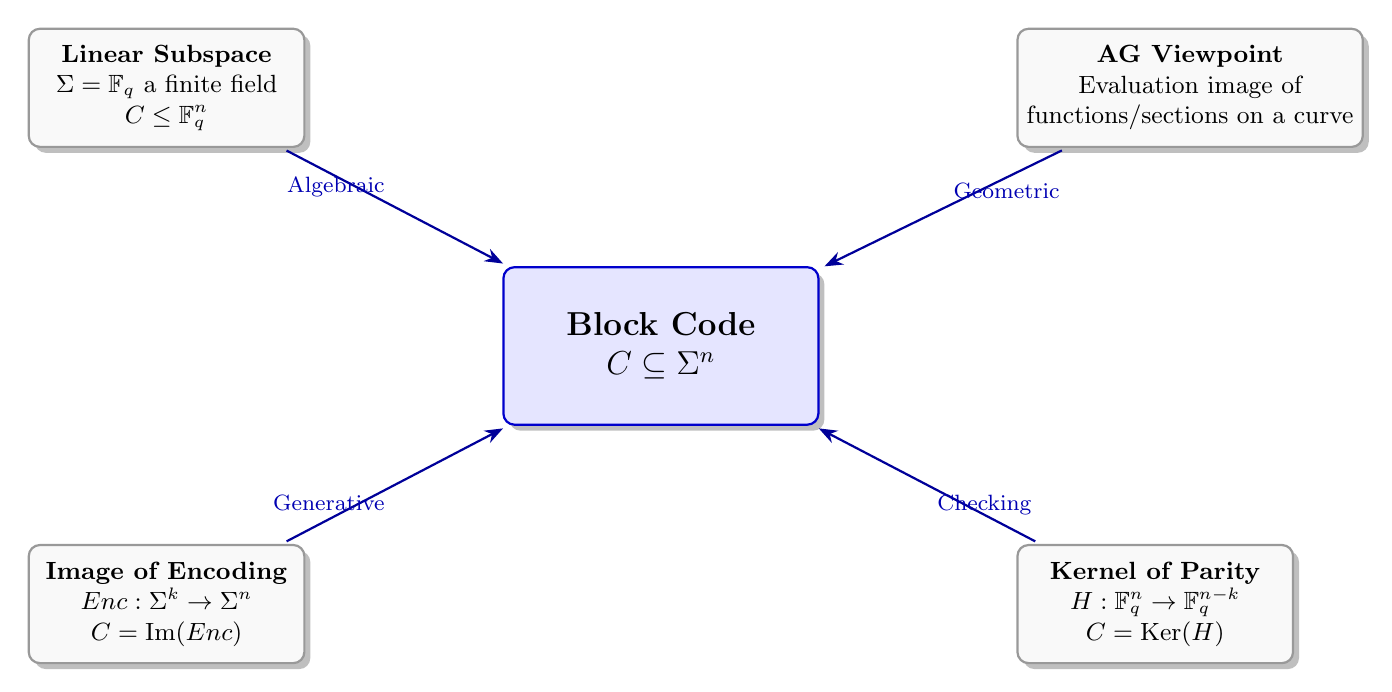
\begin{tikzpicture}[
		% Define styles for the nodes
		centerbox/.style={
			rectangle, rounded corners, draw=blue!80!black, fill=blue!10, 
			thick, text centered, align=center, minimum height=2cm, minimum width=4cm,
			font=\large\bfseries, drop shadow
		},
		viewbox/.style={
			rectangle, rounded corners, draw=gray!80, fill=gray!5, 
			thick, text centered, align=center, minimum height=1.5cm, minimum width=3.5cm,
			font=\small, drop shadow
		},
		edge/.style={
			<-, >=Stealth, thick, draw=blue!60!black, shorten <=2pt, shorten >=2pt
		}
		]
		
		% Define the central node
		\node[centerbox] (center) {Block Code \\ $C \subseteq \Sigma^n$};
		
		% Define the surrounding nodes using correct positioning keys
		\node[viewbox, above left=1.5cm and 2.5cm of center] (subspace) {
			\textbf{Linear Subspace} \\ 
			$\Sigma = \mathbb{F}_q$ a finite field \\ 
			$C \leq \mathbb{F}_q^n$
		};
		
		\node[viewbox, below left=1.5cm and 2.5cm of center] (image) {
			\textbf{Image of Encoding} \\ 
			$Enc: \Sigma^k \to \Sigma^n$ \\
			$C = \text{Im}(Enc)$
		};
		
		\node[viewbox, below right=1.5cm and 2.5cm of center] (kernel) {
			\textbf{Kernel of Parity} \\ 
			$H: \mathbb{F}_q^n \to \mathbb{F}_q^{n-k}$ \\
			$C = \text{Ker}(H)$
		};
		
		\node[viewbox, above right=1.5cm and 2.5cm of center] (ag) {
			\textbf{AG Viewpoint} \\ 
			Evaluation image of \\
			functions/sections on a curve
		};
		
		% Draw connections from the views to the central node
		\draw[edge] (center) -- (subspace) node[midway, above left, font=\footnotesize, text=blue!70!black] {Algebraic};
		\draw[edge] (center) -- (image) node[midway, below left, font=\footnotesize, text=blue!70!black] {Generative};
		\draw[edge] (center) -- (kernel) node[midway, below right, font=\footnotesize, text=blue!70!black] {Checking};
		\draw[edge] (center) -- (ag) node[midway, above right, font=\footnotesize, text=blue!70!black] {Geometric};
		
	\end{tikzpicture}
	
\end{document}